\documentclass[11pt]{article}

% ---------- Page setup ----------
\usepackage[letterpaper,margin=1in]{geometry}
\usepackage[utf8]{inputenc}
\usepackage[T1]{fontenc}

% ---------- Typography / structure ----------
\usepackage{titlesec}
\usepackage{enumitem}
\usepackage{xcolor}
\usepackage{array}
\usepackage{longtable}
\usepackage{booktabs}
\usepackage{hyperref}
\usepackage{fancyhdr}
\usepackage{graphicx}
\usepackage{caption}
\captionsetup{font={small,it},labelfont=bf,skip=4pt}

\titleformat{\section}{\normalfont\Large\bfseries}{\thesection}{0.6em}{}
\titleformat{\subsection}{\normalfont\large\bfseries}{\thesubsection}{0.6em}{}
\titleformat{\subsubsection}{\normalfont\normalsize\bfseries}{}{0em}{}
\titlespacing*{\section}{0pt}{1.6em}{0.8em}
\titlespacing*{\subsection}{0pt}{1.2em}{0.5em}
\titlespacing*{\subsubsection}{0pt}{1.0em}{0.4em}

\pagestyle{fancy}
\fancyhf{}
\fancyfoot[C]{\thepage}
\renewcommand{\headrulewidth}{0pt}

\hypersetup{
  colorlinks=true,
  linkcolor=black,
  urlcolor=black,
  pdftitle={Database Design Specification - Orbit Eats}
}

% Guidance/placeholder text style
\newcommand{\guidance}[1]{\textit{\textcolor{gray!65!black}{#1}}}

% Ragged-right column type for narrow table cells
\newcolumntype{L}[1]{>{\raggedright\arraybackslash}p{#1}}

% Allow line breaks after underscores in long identifiers
\let\oldunderscore\_
\renewcommand{\_}{\oldunderscore\allowbreak}

\setlength{\parindent}{0pt}
\setlength{\parskip}{0.6em}

\title{\bfseries Database Design Specification}
\author{}
\date{}

\begin{document}

\begin{center}
  {\Huge\bfseries Database Design Specification}\\[0.4em]
  {\large Orbit Eats --- Delivery Restaurant Management System}
\end{center}

\vspace{1.5em}

% ============================================================
\section{Introduction}
% ============================================================

\subsection{Project Title}
Orbit Eats

\subsection{Objective}
To design and implement a relational database that centralizes order, menu, ingredient, and supplier management for a delivery-based restaurant, applying theoretical database concepts to a real scenario.

\subsection{Description}
The system tracks customers, menu products with their ingredient recipes, ingredient stock, suppliers, and orders, allowing kitchen and delivery staff to manage order fulfillment from placement to delivery and restaurant management to monitor ingredient stock levels and generate sales and supplier reports.

\subsection{Scope}
Includes order management, menu and recipe tracking, ingredient inventory control, supplier sourcing, and delivery staff assignment. Excludes payment processing and a graphical user interface --- database operations are exposed only through an API, and payments are handled outside this system.

\subsection{Method}
Requirements gathered from restaurant operations (orders, kitchen, delivery, and purchasing) $\rightarrow$ conceptual ER modeling $\rightarrow$ logical schema design normalized to 3NF $\rightarrow$ validation against sample order and reporting scenarios $\rightarrow$ test case design and execution.

\subsection{Deliverables}
\begin{itemize}[leftmargin=1.4em, itemsep=0.2em]
  \item Database requirements document
  \item Conceptual data model (ER diagram)
  \item Logical data model (relational schema, data dictionary)
  \item Implementation of the database (containerized MySQL instance with API access)
  \item Test case suite and results
\end{itemize}

\subsection{Team Members}

\begin{longtable}{@{}p{3.5cm}p{3.5cm}p{6.5cm}@{}}
\toprule
\textbf{Name} & \textbf{Role} & \textbf{Responsibility} \\
\midrule
\endhead
Javier Herdoiza & Project Lead & Requirements gathering, ER modeling, relational schema design, data dictionary \\[0.6em]
Ismael Cifuentes & Database Designer & Database implementation, API integration, test case design and execution \\[0.6em]
\bottomrule
\end{longtable}

% ============================================================
\section{Project Requirements}
% ============================================================

\subsection{Functional Requirements Description}

\begin{longtable}{@{}p{2cm}p{9.5cm}p{2cm}@{}}
\toprule
\textbf{ID} & \textbf{Requirement Description} & \textbf{Priority} \\
\midrule
\endhead
FR-01 & Staff shall be able to register a new customer with name, address, phone, and email. & High \\[0.6em]
FR-02 & The system shall record each order together with the customer who placed it, the products and quantities included, the delivery address, and the order status (received, preparing, on the way, delivered, or cancelled). & High \\[0.6em]
FR-03 & The system shall store, for each product, the list of ingredients and quantities required to prepare it. & High \\[0.6em]
FR-04 & The system shall track the current stock level of each ingredient and flag ingredients that fall below their minimum stock threshold. & Medium \\[0.6em]
FR-05 & The system shall record, for each ingredient, the suppliers that provide it along with purchase price and last purchase date. & Medium \\[0.6em]
FR-06 & The system shall record the price of each product at the moment of purchase, independent of later changes to the product's base price. & Medium \\[0.6em]
\bottomrule
\end{longtable}

\subsection{Non-Functional Requirements Description}

\begin{longtable}{@{}p{2cm}p{9.5cm}p{2cm}@{}}
\toprule
\textbf{ID} & \textbf{Requirement Description} & \textbf{Category} \\
\midrule
\endhead
NFR-01 & The system shall support at least 20 concurrent order submissions without noticeable slowdown, covering peak lunch and dinner hours. & Performance \\[0.6em]
NFR-02 & Customer personal data (address, phone, email) shall be protected against unauthorized API access through authentication. & Security \\[0.6em]
NFR-03 & The system shall be available at least 99\% of the restaurant's operating hours. & Availability \\[0.6em]
\bottomrule
\end{longtable}

% ============================================================
\section{Database Design}
% ============================================================

\subsection{Conceptual Model}

\begin{figure}[h!]
  \centering
  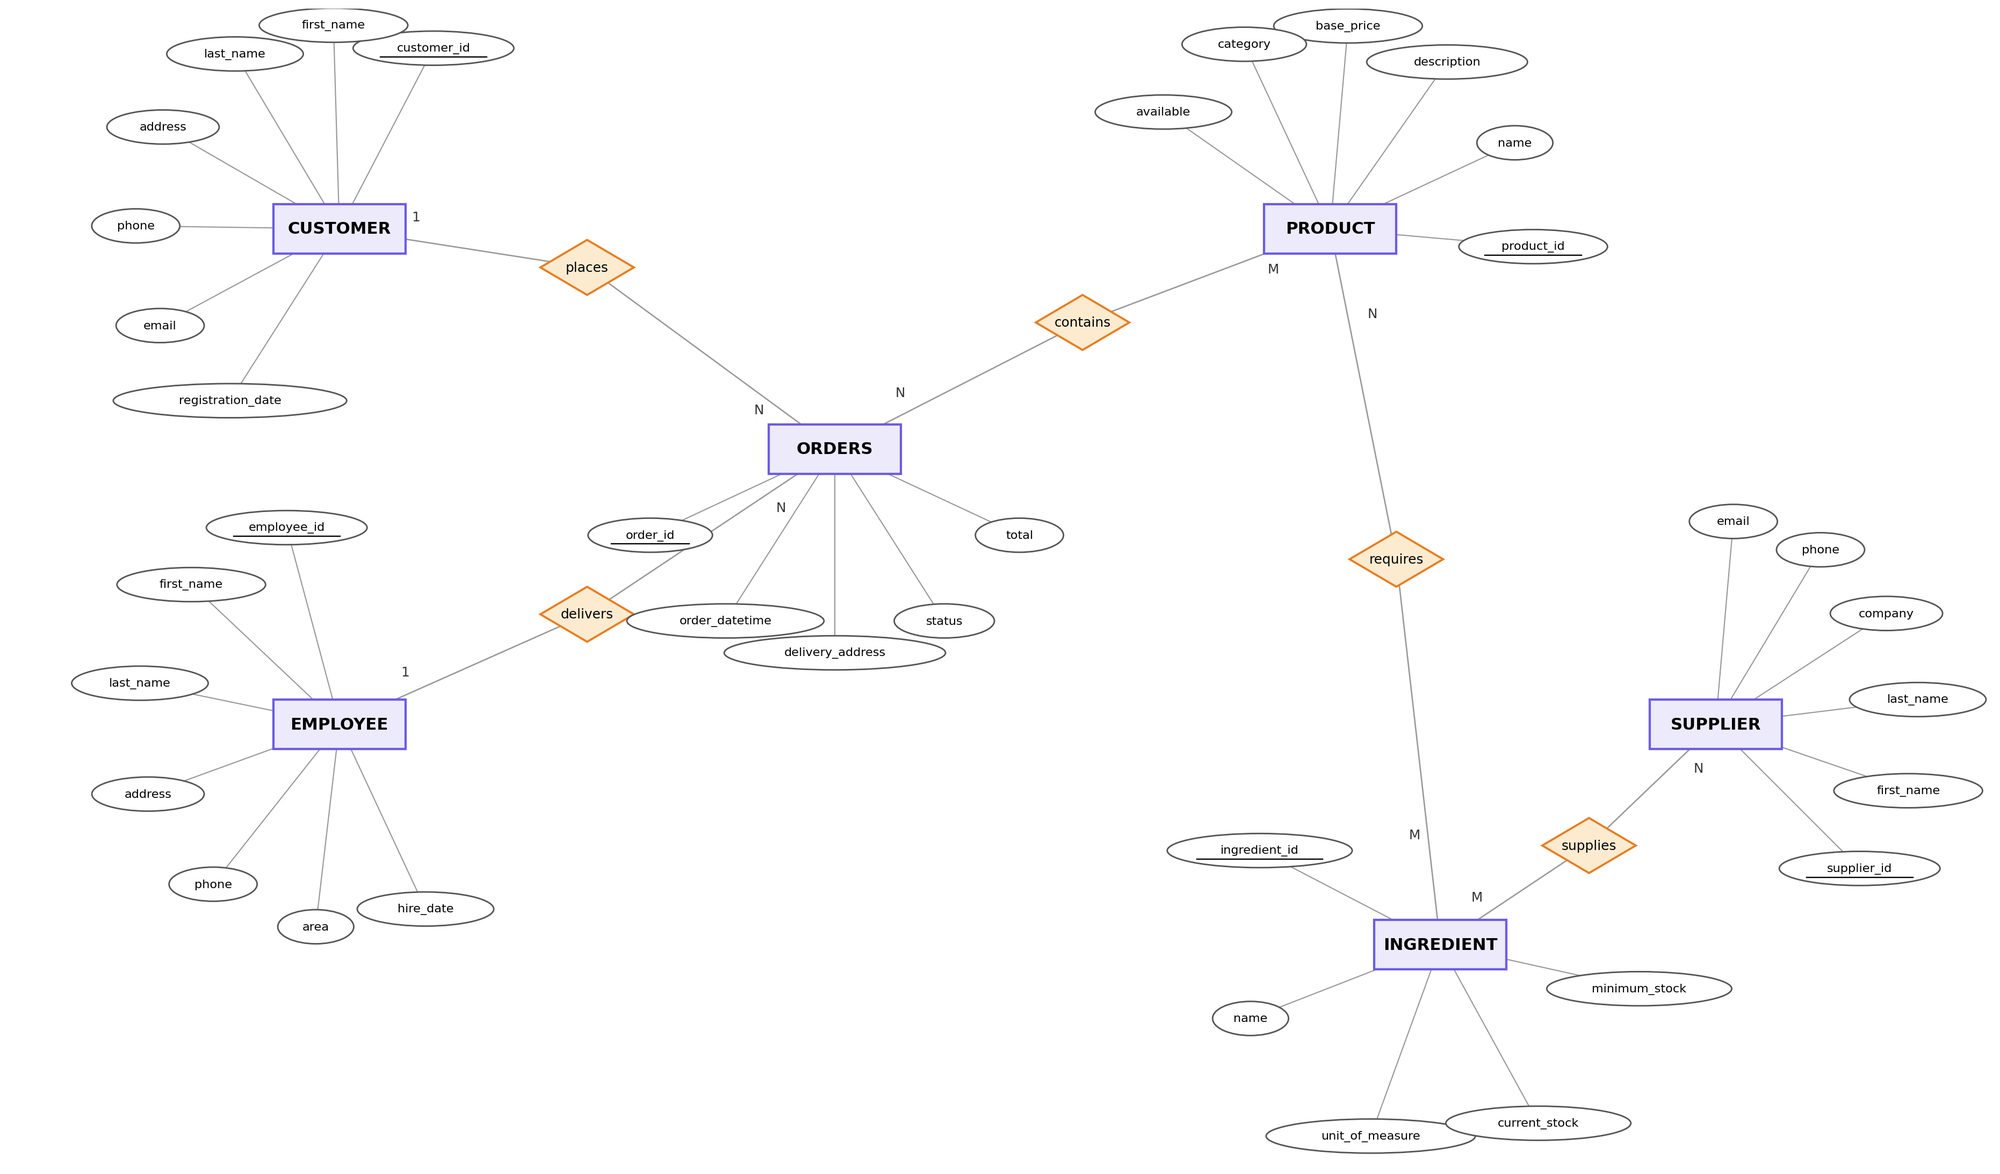
\includegraphics[width=0.98\textwidth]{images/conceptual_erd.png}
  \caption{Conceptual model --- Orbit Eats. Customer, Employee, Supplier, Ingredient, Product, and Orders are the core entities; ``requires,'' ``supplies,'' and ``contains'' are many-to-many relationships, resolved by the Product\_Ingredient, Supply, and Order\_Detail tables, respectively, in the logical model.}
\end{figure}

\vspace{0.5em}
\textbf{Entities}

\begin{longtable}{@{}p{3.5cm}p{10cm}@{}}
\toprule
\textbf{Entity} & \textbf{Description} \\
\midrule
\endhead
Customer & A registered person who places delivery orders. \\[0.6em]
Employee & A restaurant staff member, including those assigned to deliver orders. \\[0.6em]
Supplier & A company or contact that provides ingredients to the restaurant. \\[0.6em]
Ingredient & A raw item used in preparing menu products, tracked by stock level. \\[0.6em]
Product & A menu item available for order. \\[0.6em]
Orders & A customer's request for one or more products, tracked from placement to delivery. \\[0.6em]
\bottomrule
\end{longtable}

\textbf{Relationships}

\begin{longtable}{@{}p{4cm}p{2.5cm}p{7cm}@{}}
\toprule
\textbf{Relationship} & \textbf{Cardinality} & \textbf{Description} \\
\midrule
\endhead
Customer --- Orders (places) & 1:N & A customer can place many orders; each order belongs to one customer. \\[0.6em]
Employee --- Orders (delivers) & 1:N & An employee can deliver many orders; each order is delivered by at most one employee. \\[0.6em]
Orders --- Product (contains) & M:N & An order can include many products; a product can appear in many orders. \\[0.6em]
Product --- Ingredient (requires) & M:N & A product requires several ingredients; an ingredient is used in several products. \\[0.6em]
Supplier --- Ingredient (supplies) & M:N & A supplier can provide several ingredients; an ingredient can be sourced from several suppliers. \\[0.6em]
\bottomrule
\end{longtable}

\clearpage
\subsection{Logical Model}
\label{sec:logical-model}

\begin{figure}[h!]
  \centering
  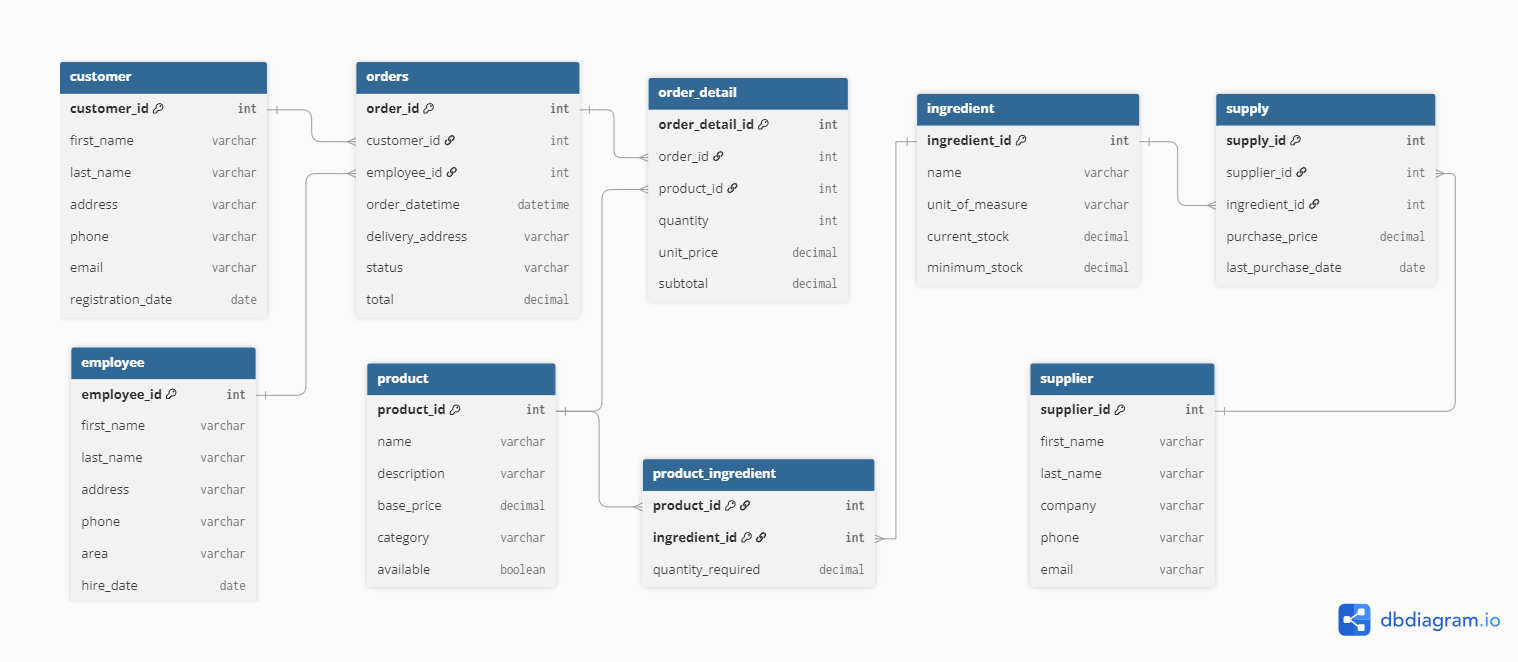
\includegraphics[width=\textwidth]{images/logical_erd.png}
  \caption{Logical model --- Orbit Eats (relational schema). The many-to-many relationships from the conceptual model are resolved by three associative tables: Order\_Detail (Orders--Product), Product\_Ingredient (Product--Ingredient), and Supply (Supplier--Ingredient).}
\end{figure}

The schema is normalized to 3NF: every non-key attribute depends only on its table's primary key, and no repeating groups or transitive dependencies remain (e.g., order line items live in \texttt{order\_detail} rather than as repeated columns in \texttt{orders}). Two columns are stored on purpose even though they can be calculated: \texttt{order\_detail.subtotal} (quantity $\times$ unit price) and \texttt{orders.total} (sum of the order's subtotals). They are written once when the order is created, so sales reports do not have to recalculate every past order. Full column detail is in Annex A; naming follows the rules in Annex B.

% ============================================================
\section{Test Cases}
\label{sec:test-cases}
% ============================================================

The test cases below validate the design against the requirements in Section~2. Functional test cases (TC-01 to TC-08) are SQL scripts run directly on the database after loading the schema and a small set of sample data (2 employees, 2 products, 4 ingredients, 2 suppliers). They were executed on MySQL~8 running in Docker and all returned the expected result. Non-functional test cases (TC-09 to TC-11) were executed on the containerized deployment with the API running: TC-09 and TC-10 with the script \texttt{test\_api.py}, and TC-11 by restarting the container.

{\footnotesize\setlength{\tabcolsep}{4pt}
\begin{longtable}{@{}L{1.1cm}L{1.2cm}L{2.5cm}L{2.6cm}L{2.9cm}L{2.6cm}L{1.3cm}@{}}
\toprule
\textbf{Test ID} & \textbf{Req. ID} & \textbf{Description} & \textbf{Precondi\-tions} & \textbf{Steps} & \textbf{Expected Result} & \textbf{Status} \\
\midrule
\endhead
TC-01 & FR-01 & Register a new customer with all required data. & Schema loaded; email \texttt{ana.lopez@} \texttt{mail.com} not registered. & \texttt{INSERT INTO customer} with name, address, phone and email; then \texttt{SELECT} by email. & One row returned; \texttt{customer\_id} generated and \texttt{registration\_date} set to today. & Pass \\[0.8em]
TC-02 & FR-01 & Reject a customer whose email already exists. & TC-01 executed. & \texttt{INSERT INTO customer} with a different name and the same email. & Error 1062: duplicate entry for key \texttt{uq\_customer\_email}; no row inserted. & Pass \\[0.8em]
TC-03 & FR-02 & Record an order with its products, address and status. & Customer 1, employee 1 and products 1--2 exist. & Insert order (status \texttt{received}); insert 2 lines in \texttt{order\_detail}; update \texttt{total}; query with \texttt{JOIN}. & 2 detail lines (2 burgers = 13.00, 1 fries = 2.00); total = 15.00; status = received. & Pass \\[0.8em]
TC-04 & FR-02 & Reject an invalid status and an order for a non-existent customer. & Order 1 exists; customer 999 does not exist. & \texttt{UPDATE orders SET status='lost'}; \texttt{INSERT INTO orders} with \texttt{customer\_id = 999}. & First: \texttt{ck\_orders\_status} fails. Second: error 1452, \texttt{fk\_orders\_customer} fails. & Pass \\[0.8em]
TC-05 & FR-03 & List the recipe (ingredients and quantities) of a product. & Recipe of ``Classic Burger'' loaded in \texttt{product\_ingredient}. & \texttt{SELECT} joining \texttt{product}, \texttt{product\_ingredient} and \texttt{ingredient} where product = ``Classic Burger''. & 3 rows: Burger bun, Beef patty and Cheese slice, 1 unit each. & Pass \\[0.8em]
TC-06 & FR-04 & Flag ingredients below their minimum stock. & Beef patty: stock 8, minimum 15. Other ingredients above minimum. & \texttt{SELECT ... FROM ingredient WHERE current\_stock < minimum\_stock}. & Only 1 row: Beef patty (8.00 / 15.00). & Pass \\[0.8em]
TC-07 & FR-05 & Show the suppliers of an ingredient and avoid duplicate supplier--ingredient pairs. & Supplier 1 supplies Beef patty at 1.20 (2026-11-02). & \texttt{SELECT} joining \texttt{supply}, \texttt{supplier} and \texttt{ingredient}; then insert the same pair again. & Query shows Carnes del Valle, 1.20, 2026-11-02. Second insert fails on \texttt{uq\_supply\_supplier\_ingredient}. & Pass \\[0.8em]
TC-08 & FR-06 & Keep the price paid after the product's base price changes. & TC-03 executed (burger sold at 6.50). & \texttt{UPDATE product SET base\_price = 7.00}; compare \texttt{base\_price} with \texttt{order\_detail.unit\_price}. & Current price = 7.00; price paid in order 1 = 6.50 (unchanged). & Pass \\[0.8em]
TC-09 & NFR-01 & Handle 20 orders submitted at the same time. & API and MySQL container running; sample data loaded. & Python script with 20 threads, each sending \texttt{POST /orders} at the same moment; measure response times. & All 20 orders stored with their details; no errors; each response in under 2 s (measured: 0.32 s). & Pass \\[0.8em]
TC-10 & NFR-02 & Block access to customer data without authentication. & API running with authentication enabled; one valid user. & \texttt{GET /customers} without token; repeat with an invalid token; repeat with a valid token. & No token / invalid token: HTTP 401 and no data. Valid token: HTTP 200 with the customer list. & Pass \\[0.8em]
TC-11 & NFR-03 & Recover the service and keep the data after a container restart. & Container started with \texttt{--restart unless-stopped} and a Docker volume mounted on \texttt{/var/lib/mysql}. & Count rows in \texttt{orders}; run \texttt{docker restart}; wait; count rows again and call the API. & Service available again in under 1 minute; same number of orders before and after. & Pass \\[0.8em]
\bottomrule
\end{longtable}
}

% ============================================================
\section{Disclaimer}
% ============================================================

The database design produced from this specification will be evaluated against compliance with the test cases defined in Section~\ref{sec:test-cases}. Acceptance of the design is contingent on the successful execution of every test case listed; any test case that fails must be remediated and re-tested before the design is considered complete and approved.

\clearpage
% ============================================================
\section{Use of Generative AI}
% ============================================================

Generative AI was used in preparing part of this document. Its use is described below and every prompt is recorded in Section~6.2.

\subsection{Role of Generative AI}
The project idea, the requirements (Section~2), and the conceptual and logical models (Section~3) were developed by the team in the first part of the project; the logical diagram was drawn with dbdiagram.io. For this second part, generative AI (Claude) was used to draft the test cases in Section~4, the SQL and Python scripts used to run them, to correct and extend the team's Flask API used in the non-functional tests, the data dictionary in Annex~A (data types, sizes and constraints), the adjustment of the naming conventions in Annex~B to the existing schema, and the formatting of the document in \LaTeX{}. The AI worked from the team's own diagrams, the course notes and the bibliography given by the professor. All AI-assisted content was reviewed by the team, and every test case was executed by the team on its own environment before being marked as \textit{Pass}. Final design decisions remain the responsibility of the authors.

\subsection{Prompts, Model, and Version Used}

{\small
\begin{longtable}{@{}L{2.6cm}L{5.2cm}L{2.4cm}L{2.1cm}L{1.9cm}@{}}
\toprule
\textbf{Section / Task} & \textbf{Prompt Used} & \textbf{Generative Model} & \textbf{Version} & \textbf{Date} \\
\midrule
\endhead
Sections 4, 6, 7, Annex A, Annex B; SQL test scripts & ``Necesito finalizar el proyecto grupal de bases de datos, revisa el ejemplo y el template para látex. En base a todo lo que se ha visto en clase [...] realiza los puntos faltantes con lo aprendido en clase, que no sea muy complejo o difícil de explicar [...]'' (with the template, the example document and the first part of the project attached) & Claude Opus 5.5 & claude-opus-5-5 & 2026-11-15 \\[0.6em]
API correction and extension; API tests (TC-09, TC-10) & ``Esto es lo que estaba trabajando mi compañero: [Flask API code] Dame el paso a paso para finalizar y realizar la entrega [...]'' & Claude Opus 5.5 & claude-opus-5-5 & 2026-11-16 \\[0.6em]
\bottomrule
\end{longtable}
}

% ============================================================
\section{References}
% ============================================================

\begin{enumerate}[leftmargin=1.4em, itemsep=0.5em]
  \item Silberschatz, A., Korth, H. F., \& Sudarshan, S. (2019). \textit{Database System Concepts} (7th ed.). McGraw-Hill Education.
  \item Teate, R. M. P. (2021). \textit{SQL for Data Scientists: A Beginner's Guide for Building Datasets for Analysis}. Wiley.
  \item Oracle Corporation. (2024). \textit{MySQL 8.0 Reference Manual}. \url{https://dev.mysql.com/doc/refman/8.0/en/}
  \item Docker Inc. (2024). \textit{Docker Documentation: Volumes and restart policies}. \url{https://docs.docker.com/}
  \item Pallets. (2024). \textit{Flask Documentation}. \url{https://flask.palletsprojects.com/}
  \item Pallets. (2024). \textit{Flask-SQLAlchemy Documentation}. \url{https://flask-sqlalchemy.readthedocs.io/}
  \item Holistics Software. (2024). \textit{dbdiagram.io --- Database relationship diagrams design tool}. \url{https://dbdiagram.io/}
\end{enumerate}

\clearpage
% ============================================================
\section*{Annex A: Data Dictionary}
% ============================================================
\addcontentsline{toc}{section}{Annex A: Data Dictionary}

Column-level detail for every table in the logical model (see Section~\ref{sec:logical-model}), following the naming rules in Annex~B. Unless marked \textit{NULL}, every column is \texttt{NOT NULL}. All primary keys of type \texttt{INT} use \texttt{AUTO\_INCREMENT}, except in \texttt{product\_ingredient}, whose key is composite.

{\small
\begin{longtable}{@{}L{2.5cm}L{2.7cm}L{2.6cm}L{2.6cm}L{3.7cm}@{}}
\toprule
\textbf{Table} & \textbf{Column} & \textbf{Data Type} & \textbf{Key} & \textbf{Description} \\
\midrule
\endhead
customer & customer\_id & INT & PK & Unique identifier of the customer. \\[0.4em]
customer & first\_name & VARCHAR(50) & & Customer's first name. \\[0.4em]
customer & last\_name & VARCHAR(50) & & Customer's last name. \\[0.4em]
customer & address & VARCHAR(150) & & Default delivery address. \\[0.4em]
customer & phone & VARCHAR(15) & & Contact phone number. \\[0.4em]
customer & email & VARCHAR(100) & UNIQUE & Email address; cannot repeat. \\[0.4em]
customer & registration\_date & DATE & & Date the customer was registered (default: current date). \\[0.4em]
\midrule
employee & employee\_id & INT & PK & Unique identifier of the employee. \\[0.4em]
employee & first\_name & VARCHAR(50) & & Employee's first name. \\[0.4em]
employee & last\_name & VARCHAR(50) & & Employee's last name. \\[0.4em]
employee & address & VARCHAR(150) & & Home address (NULL allowed). \\[0.4em]
employee & phone & VARCHAR(15) & & Contact phone number. \\[0.4em]
employee & area & VARCHAR(20) & CHECK & Work area: \texttt{kitchen}, \texttt{delivery} or \texttt{admin}. \\[0.4em]
employee & hire\_date & DATE & & Date the employee was hired. \\[0.4em]
\midrule
orders & order\_id & INT & PK & Unique identifier of the order. \\[0.4em]
orders & customer\_id & INT & FK $\rightarrow$ customer & Customer who placed the order. \\[0.4em]
orders & employee\_id & INT & FK $\rightarrow$ employee & Employee who delivers the order (NULL until assigned). \\[0.4em]
orders & order\_datetime & DATETIME & & Date and time the order was placed (default: now). \\[0.4em]
orders & delivery\_address & VARCHAR(150) & & Address where this order is delivered. \\[0.4em]
orders & status & VARCHAR(20) & CHECK & \texttt{received}, \texttt{preparing}, \texttt{on\_the\_way}, \texttt{delivered} or \texttt{cancelled} (default: received). \\[0.4em]
orders & total & DECIMAL(10,2) & CHECK & Sum of the order's subtotals; must be $\geq 0$. \\[0.4em]
\midrule
order\_detail & order\_detail\_id & INT & PK & Unique identifier of the order line. \\[0.4em]
order\_detail & order\_id & INT & FK $\rightarrow$ orders & Order this line belongs to. \\[0.4em]
order\_detail & product\_id & INT & FK $\rightarrow$ product & Product ordered. \\[0.4em]
order\_detail & quantity & INT & CHECK & Units ordered; must be $> 0$. \\[0.4em]
order\_detail & unit\_price & DECIMAL(8,2) & & Product price at the moment of purchase (FR-06). \\[0.4em]
order\_detail & subtotal & DECIMAL(10,2) & & quantity $\times$ unit\_price. \\[0.4em]
\midrule
product & product\_id & INT & PK & Unique identifier of the menu product. \\[0.4em]
product & name & VARCHAR(80) & & Product name shown on the menu. \\[0.4em]
product & description & VARCHAR(255) & & Short description (NULL allowed). \\[0.4em]
product & base\_price & DECIMAL(8,2) & CHECK & Current menu price; must be $> 0$. \\[0.4em]
product & category & VARCHAR(30) & & Menu category (e.g., burgers, sides, drinks). \\[0.4em]
product & available & BOOLEAN & & TRUE if the product can be ordered (default: TRUE). \\[0.4em]
\midrule
product\_ingredient & product\_id & INT & PK, FK $\rightarrow$ product & Product that uses the ingredient. \\[0.4em]
product\_ingredient & ingredient\_id & INT & PK, FK $\rightarrow$ ingredient & Ingredient used in the product. \\[0.4em]
product\_ingredient & quantity\_required & DECIMAL(8,2) & CHECK & Amount of the ingredient needed for one unit of the product; must be $> 0$. \\[0.4em]
\midrule
ingredient & ingredient\_id & INT & PK & Unique identifier of the ingredient. \\[0.4em]
ingredient & name & VARCHAR(60) & UNIQUE & Ingredient name; cannot repeat. \\[0.4em]
ingredient & unit\_of\_measure & VARCHAR(10) & & Unit used for stock (e.g., kg, l, unit). \\[0.4em]
ingredient & current\_stock & DECIMAL(10,2) & CHECK & Quantity currently in stock; must be $\geq 0$. \\[0.4em]
ingredient & minimum\_stock & DECIMAL(10,2) & CHECK & Threshold below which the ingredient is flagged (FR-04); must be $\geq 0$. \\[0.4em]
\midrule
supply & supply\_id & INT & PK & Unique identifier of the supply record. \\[0.4em]
supply & supplier\_id & INT & FK $\rightarrow$ supplier; UNIQUE (with ingredient\_id) & Supplier that provides the ingredient. \\[0.4em]
supply & ingredient\_id & INT & FK $\rightarrow$ ingredient & Ingredient provided. \\[0.4em]
supply & purchase\_price & DECIMAL(8,2) & CHECK & Price paid to this supplier per unit; must be $> 0$. \\[0.4em]
supply & last\_purchase\_date & DATE & & Date of the last purchase from this supplier. \\[0.4em]
\midrule
supplier & supplier\_id & INT & PK & Unique identifier of the supplier. \\[0.4em]
supplier & first\_name & VARCHAR(50) & & Contact person's first name. \\[0.4em]
supplier & last\_name & VARCHAR(50) & & Contact person's last name. \\[0.4em]
supplier & company & VARCHAR(80) & & Supplier company name. \\[0.4em]
supplier & phone & VARCHAR(15) & & Contact phone number. \\[0.4em]
supplier & email & VARCHAR(100) & & Contact email (NULL allowed). \\[0.4em]
\bottomrule
\end{longtable}
}

\clearpage
% ============================================================
\section*{Annex B: Naming Conventions}
% ============================================================
\addcontentsline{toc}{section}{Annex B: Naming Conventions}

The following rules were applied to every element of the schema. The only deviation is the table \texttt{orders}, which is plural because \texttt{ORDER} is a reserved word in SQL (\texttt{ORDER BY}); using it as a table name would require quoting it in every query.

{\small
\begin{longtable}{@{}L{2.5cm}L{7.0cm}L{4.1cm}@{}}
\toprule
\textbf{Element} & \textbf{Naming Rule} & \textbf{Example} \\
\midrule
\endhead
Entity / table & Singular noun, snake\_case, all lowercase (exception: \texttt{orders}, see above) & \texttt{customer}, \texttt{ingredient} \\[0.6em]
Associative table & Name of the two tables joined (\texttt{<table1>\_<table2>}) or a noun that describes the relationship & \texttt{product\_ingredient}, \texttt{order\_detail}, \texttt{supply} \\[0.6em]
Attribute / column & snake\_case, descriptive noun; avoid abbreviations unless standardized & \texttt{first\_name}, \texttt{order\_datetime} \\[0.6em]
Primary key & Column named \texttt{<table>\_id}; constraint named \texttt{pk\_<table>} & \texttt{customer\_id} \textperiodcentered{} \texttt{pk\_customer} \\[0.6em]
Foreign key & Same name as the referenced primary key (\texttt{<ref>\_id}); constraint named \texttt{fk\_<table>\_<ref>} & \texttt{customer\_id} (in \texttt{orders}) \textperiodcentered{} \texttt{fk\_orders\_customer} \\[0.6em]
Unique constraint & \texttt{uq\_<table>\_<col(s)>} & \texttt{uq\_customer\_email}, \texttt{uq\_supply\_supplier\_ingredient} \\[0.6em]
Check constraint & \texttt{ck\_<table>\_<rule>} & \texttt{ck\_orders\_status}, \texttt{ck\_product\_base\_price\_positive} \\[0.6em]
Index & \texttt{idx\_<table>\_<col(s)>} & \texttt{idx\_orders\_customer\_id} \\[0.6em]
\bottomrule
\end{longtable}
}

\end{document}
